
\section{Lecture 19: Rotating rigid bodies, inertia and axis theorems}

This week is mostly if not exclusively about rotation and related concepts such as rotational energy, moments of inertia, angular momentum, torques, etc.\\
To get started, we begin by finding some equations for rotational motion, very similar to the kinematics equations for linear motion that we first saw in week one of the course.

Say an object is moving along a circular path, at some angular velocity $\omega$. It has a tangential speed $v$, which always points tangent to its position on the circle. So far, nothing has changed compared to uniform circular motion.

However, we can now allow $v$ to change in magnitude. Previously, only the direction of the velocity vector $\vec{v}$ changed, in order to stay along the circle. The tangential speed $v$ was always the the same in uniform circular motion. That is what we now change.

$v = \omega R$, as we have seen before. $\omega = \dot{\theta}$ (that is, the first time derivative of theta), so $v = \dot{\theta} R$ also.\\
If we take the time derivative of the angular velocity $\omega$, we find the angular acceleration, $\alpha = \dot{\omega} = \ddot{\theta}$. We use the symbol lowercase alpha for angular acceleration, and the units are $\text{rad/s}^2$.

There are now two accelerations that this object experiences. One is the radial acceleration, that is, the inwards (centripetal) acceleration $a_c$ required for it to change direction so that the motion is circular. There is also the tangential acceleration $\alpha$, which changes the angular velocity of the object as it moves along the circle.\\
Note that the two have different units, however. The centripetal acceleration will, in MKS units, be in $\text{m/s}^2$, while the angular acceleration is in $\text{rad/s}^2$. In order for them to have the same set of units, we need to convert the angular acceleration tangential acceleration via $a_{tan} = \alpha R$. Only then can we add the two to find the net acceleration vector.

By making some very simple substitutions, we can use the same equations we used previously. We replace $x$ with $\theta$, $v$ with $\omega$ and $a$ with $\alpha$, and that's it! These equations can be derived the same way as the kinematics equations, by assuming a constant angular acceleration $\alpha$ and integrating that with respect to time.

For the angular velocity, we find

\begin{equation}
\omega = \int \alpha \mathop{dt} = \omega_0 + \alpha t
\end{equation}

$\omega_0$ appears from the constant of integration. We can then integrate this to find the angle as a function of time:

\begin{equation}
\theta = \int (\omega_0 + \alpha t) \mathop{dt} = \theta_0 + \omega_0 t + \frac{1}{2} \alpha t^2
\end{equation}

Again we have a constant of integration, which is the initial angle $\theta_0$.

We can then use these equations in all cases where there is a \emph{constant} angular acceleration. In other cases, integrals are the way to go.

The direction of angular velocity (and acceleration) is found by using the right-hand rule; see the part on vector mathematics for more information. In short, you can curl the fingers of your \emph{right} hand (the left hand will give the opposite answer! The convention to use the right hand for consistency) along the rotation, and your thumb will point along the vector's direction, perpendicular to the actual rotational movement.\\
Alternatively, you can use the professor's preferred version, the right-hand corkscrew rule. Imagine turning a corkscrew clockwise: it goes into the screen. Turn it counterclockwise, and it goes out of the screen.

For accelerations, beware that you need to curl your fingers along the acceleration, not along the current rotation! The two are the same if the rotation speed is increasing, but opposite if it is decreasing!\\
For example, if the current rotation is counterclockwise at 100 rad/s, the angular velocity vector points ``out of the screen'' using the right hand rule.\\
If the rotation is speeding up, the acceleration vector is also in this direction.\\
However, if it is slowing down, so that it will eventually come to a halt and reverse, the acceleration is in the opposite direction. We curl our fingers opposite the motion, so clockwise in this case, which means you need to turn your hand (rather awkwardly) to curl your fingers, and your thumb then points inwards. In this case, the right-hand corkscrew rule is certainly easier.

\subsection{Moment of inertia and rotational kinetic energy}

Let's now calculate the kinetic energy stored in rotating objects. First, let's limit ourselves to a simple disk, rotating along a perpendicular axis.

The disk has a mass $m$, and a radius $R$, and rotates with angular velocity $\omega$ (that may or may not be constant).

In order to find the rotational kinetic energy, we add up the kinetic energy of each tiny portion of the disk. Say we divide it into tiny pieces, each with a mass $m_i$, at a distance $r_i$ from the center of the disk.  It is clear that the elements very near the edge of the disk move at a high velocity, while ones near the center barely move at all, making tiny tiny circles.

The kinetic energy of one such mass piece is simply $\displaystyle K_i = \frac{1}{2} m_i v_i^2$, where we can find the velocity as $v_i = \omega r_i$ -- something that always holds for circular motion. Because of this relationship, we can re-write the kinetic energy in turns of $\omega r_i$ instead of $v_i$, and find

\begin{equation}
K_i = \frac{1}{2} m_i \omega^2 r_i^2
\end{equation}

This is a useful change, since $v_i$ depends on the location of the element, as noted above. $\omega$ is a constant for the disk, however, so we now have the kinetic energy in terms of our elements $m_i$ and their distances from the center $r_i$ only.\\
The total kinetic energy is then the sum

\begin{equation}
K = \sum_i \frac{1}{2} m_i \omega^2 r_i^2 = \frac{1}{2} \omega^2 \sum_i m_i r_i^2
\end{equation}

We can factor out the $\displaystyle \frac{1}{2} \omega^2$, since it is the same for all elements. The sum we have above is known as the \emph{moment of inertia}, $I$ (not to be confused with impulse, which is unrelated).

\begin{equation}
I_C = \sum_i m_i r_i^2
\end{equation}

This is the moment of inertia about the center of the disk, which is why there is a $C$ above; more on that in a second. However, now that we have a name for this sum, we can write the kinetic energy in a form very similar to the one we already know:

\begin{equation}
K = \frac{1}{2} I_C \omega^2
\end{equation}

$\omega$ takes the place of $v$, as we mentioned earlier regarding the kinematics equations, but note that $I_C$ takes the place of the mass $m$. The mass (inertial mass) of an object is a measure of its inertia, that is, how hard it is to accelerate it. The greater the mass, the greater the force required for a certain acceleration.\\
The same thing can be said about the moment of inertia, in the case of rotational motion. The higher the moment of inertia, the harder it is to change the angular velocity of an object about an axis of rotation, so the \emph{torque} required is higher. (Torque is introduced later this week, but in short, it is sort-of the amount of twisting a force produces.)

We now know how to calculate kinetic energy, given we know the moment of inertia. The professor recommends looking those up in tables in books, rather than memorizing, since they depend not only on the shape of the object, but also on about which axis you rotate it, and whether that axis is centered or not.

Let's try to calculate that of the disk, though. Say we rotate it as mentioned, about the perpendicular axis, through its center (i.e. in the most obvious way there is). Also, let's actually model it as a cylinder, since the height may matter, so that we get a more general result. The height is $h$, radius $R$. The volume is then $\pi R^2 h$, and the density $\displaystyle \rho = \frac{M}{\pi R^2 h}$, assuming uniform density.

The derivation is fairly long if we don't skip any steps, so to be clear, I will spell many of them out. We begin with the definition of the moment of inertia, and take the limit to get an integral, via the definition of the integral:

\begin{equation}
I_C = \lim_{\Delta m_i \to 0} \sum_i r_i^2 \Delta m_i = \int r_i^2 \mathop{dm}
\end{equation}

$dm$ is given by $\rho dV$ if $\rho$ is the density, and $dV$ a small volume element. If the density is uniform, we can find $\rho$ from the total mass, divided by the volume:

\begin{equation}
\rho = \frac{M}{\pi R^2 h}
\end{equation}

Meanwhile, $dV$ can be written in terms of $dr$. We can find the volume of a cylinder by integrating infinitesimally thin cylindrical shells. They then have a thickness $dr$, and circumference $2 \pi r$. $V = h \int 2 \pi r \mathop{dr}$, so $dV = 2 \pi r h \mathop{dr}$. We finally have all the parts, so we put them together, integrate and simplify:

\begin{equation}
I_C = \int r^2 \mathop{dm} = \int r^2 \rho \mathop{dV} = \int r^2 \rho (2 \pi r h \mathop{dr}) = 2 \pi \rho h \int r^3 \mathop{dr}
\end{equation}

Make the substitution for $\rho$:

\begin{equation}
I_C = 2 \pi \left( \frac{M}{\pi R^2 h}\right) h \int_0^R r^3 \mathop{dr} = \frac{2 M}{R^2} \left(\frac{R^4}{4}\right) = \frac{M R^2}{2}
\end{equation}

So in the end, we find the moment of inertia of a cylinder (or disk) with uniform mass density, rotating around its center on an axis perpendicular to the radius, is 

\begin{equation}
I_C = \frac{1}{2} M R^2
\end{equation}

Never forget that this result is only valid for the conditions above, though! The moment of inertia for other shapes, or even the same shape but different axes or off-center rotation are all different, as we'll see rather soon. I'm starting to see why the professor didn't derive any examples in class!

What about for a sphere, again of uniform density, rotating around an axis through its center?\\
This derivation may seem very simple, but if you start from the definition for the moment of inertia of a point mass, it's actually a rather ugly triple integral. The reason is that the $r_i$ in $\int r_i^2 \mathop{dm}$ is not the distance from the sphere's center, but the distance from the \emph{axis of rotation}. Consider a point near the ``north pole'' of the sphere. It is $R$ from the center of the sphere, but much closer to the axis of rotation, so a simple integral doesn't give us the correct answer.

We can, however, derive it in terms of infinitely thin disks, now that we know the  above result. We stack an infinite number of such disks, where the top disk has approximately 0 radius, and they grow up to $R$, and then go back down to 0 near the opposite pole again. The radius of each disk, call it $x$ (since $r$ could be confusing, see above), can be found using the Pythagorean theorem. I find it a bit difficult to visualize, but I did draw it out and found the relationship $z^2 + x^2 = R^2$, where $z$ is the height above the sphere's center. That gives us $x^2 = R^2 - z^2$.

We then use a coordinate system centered on the sphere, and integrate from $z = -R$ to $z = +R$.

\begin{equation}
I_C = \int_{-R}^{R} \frac{1}{2} x^2 \mathop{dm}
\end{equation}

For a disk, $dm = \pi x^2 \rho dz$, where $dz$ is the height of the disk. (The total height of the sphere is then $z = 2R$.)

\begin{equation}
I_C = \int_{-R}^{R} \frac{1}{2} x^2 (\pi x^2 \rho \mathop{dz}) = \frac{\pi \rho}{2} \int_{-R}^{R} x^4 \mathop{dz}
\end{equation}

Finally, using the relationship for $x^2$ above -- since $x^4 = (x^2)^2$ -- and integrating from $0$ to $R$ to simplify (the problem is symmetric, so this doesn't change the answer if we multiply it by 2 also)

\begin{equation}
I_C = \frac{\pi \rho}{2} \int_{-R}^{R} (R^2 - z^2)^2 \mathop{dz} = \pi \rho \int_{0}^{R} (R^2 - z^2)^2 \mathop{dz}
\end{equation}

We substitute in $\displaystyle \rho = \frac{M}{(4/3) \pi R^3}$, which contains a divided by $\pi$ that cancels in front of the integral:

\begin{equation}
I_C = \frac{M}{(4/3) R^3} \int_{0}^{R} (R^2 - z^2)^2 \mathop{dz} = \frac{M}{(4/3) R^3} \int_{0}^{R} \left(R^4 - 2 R^2 z^2 + z^4 \right)\mathop{dz}
\end{equation}

The integral equals $\displaystyle \frac{8 R^5}{15}$, so

\begin{equation}
I_C = \frac{M}{(4/3) R^3} \left(\frac{8 R^5}{15}\right) = \frac{24 M R^2}{60} = \frac{2}{5} M R^2
\end{equation}

is the moment of inertia for a solid sphere of uniform density.

\subsection{Parallel axis theorem}

Note that the moments of inertia we've found so far are only valid along exactly one axis. That axis must always be exactly through the center of mass of the object. There are two useful theorems that we can use to find the moment of inertia about other axes.

First out is the parallel axis theorem, which we can use the find the moment of inertia for an off-center axis, that is parallel to the original one (thus the name!).\\
Unfortunately, the lecture video refuses to play properly (on the 8.01x site and on YouTube as well), so I can't grab a screenshot.

Imagine the disk rotating as before, around an axis through its center of mass. We move this axis a distance $d$ from the disk's center, so that the disk is now wobbling back and forth as it rotates. The new moment inertia for this off-center axis is

\begin{equation}
I = I_C + M d^2
\end{equation}

where $M$ is the total mass of the disk.\\
This theorem is not limited to disks, however, but works for a mass distribution of any shape, which makes it very powerful.

\subsection{Perpendicular axis theorem}

In the case where we have a very thin mass distribution, i.e. a practically 2-dimensional object, we can also use a second theorem: the \emph{perpendicular axis theorem}.

Say we have three axes, $x$, $y$ and $z$, each perpendicular to each other, going through a common point of the object. We can then relate the moments of inertia of rotations along these three axes.\\
We define the $z$ axis to be perpendicular to the object's area (since it is 2-dimensional), while the $x$ and $y$ axes are in the plane of the object. It then holds that the moment of inertia of rotation along the $z$ axis is the sum of the moments of inertia for the $x$ and $y$ axes:

\begin{equation}
I_z = I_x + I_y
\end{equation}

This can then be used in a few different cases, depending on what you know and what you want to know.

\subsection{Flywheels}

We already know that rotating objects have kinetic energy. Unlike the case of linear motion, however, it is often fairly simple to ``store'' energy in a rotating object. Linear motion would clearly mean that the object needs to move, while a rotating object can remain in one place and still store vast amounts of kinetic energy.

A rotating disk or wheel that is used to store energy is known as a \emph{flywheel}. The idea is that we can store energy and the use it up later. We will now look at one of many cases where a flywheel can be used: to store energy that is otherwise wasted as heat in the brakes of cars.

Say we are driving through the mountains, on a dangerous, narrow road, so that we must keep our speed low in order to not lose control. The car starts out 500 meters above a valley, that it is driving into (and later out of, back to another 500 meter high peak). The mass of the car is 1000 kg.

If we say the car's speed must not exceed 4 m/s (14 km/h), the kinetic energy of the car is roughly 8 kJ (or less).\\
The speed will of course increase by itself by driving downhill, so the driver constantly applies the brakes, which simply turn the kinetic energy into heat -- wasting it, in other words, in addition to causing wear on the brakes.

By the work-energy theorem, the total increase in kinetic energy, almost all of which is ultimately wasted as heat, comes from the change in gravitational potential energy $m g h$. For the numbers given, $m g h = \SI{5e6}{J}$, or 625 times the car's maximum allowed kinetic energy, due the speed limit we set.

Now consider what would happen if we used that energy to start rotating a flywheel instead. The flywheel can use magnetic bearings and be mounted in a vacuum, so that the amount of friction practically goes to zero, so that almost no energy is lost, at least not over reasonably short periods of time.

Say we give the wheel a radius of $R = 0.5$ m, and a mass $M = 200$ kg -- that gives it a moment of inertia of $\displaystyle I = \frac{1}{2} M R^2 = \SI{25}{kg m^2}$.\\
We then want the disk to store as much as possible of the 5 MJ of gravitational potential energy we could use up. We can set that equal to the kinetic energy of the disk, and find out what the angular velocity needs to be:

\begin{align}
\frac{1}{2} I \omega^2 &= m g h\\
\omega &= \sqrt{\frac{2m g h}{I}}
\end{align}

For these numbers, $\omega \approx 632$ rad/s, which is about 100 revolutions per second, or very close to 6000 rpm.

Volvo announced such a system in 2013, with a 6 kg carbon fiber disc, with a 20 cm radius. It can spin at up to 60 000 rpm, however, so let's have a quick look at the maximum energy storage, considering the much smaller dimensions and lower mass. Kinetic energy goes with $\omega^2$ so I would not be surprised if the net result was still similar to the above.

\begin{equation}
\frac{1}{2} \left(\frac{1}{2} M R^2\right) \left((\SI{1000}{Hz})(\SI{2\pi}{rad})\right)^2 = \SI{2.37e6}{J}
\end{equation}

It turns out that their system stores about half the amount of energy, though in a flywheel that is 3\% the mass, and less than half the radius.

This type of braking is useful for driving on flat ground too, of course, only that the initial energy source will likely have to be the car's engine in that case. You should still be able to store energy in a flywheel when braking, and extract it at a later time, and perhaps use it to power an electric engine.

Designing such a system is certainly not an easy task, but it can be done, and has been demonstrated. There are other issues than simply finding an efficient way of extracting and storing the energy, though, including one we might understand better at the end of this week, or next week, regarding how the rotating wheel will very strongly resist changes in its motion.

``A car has a flywheel (a disk of radius $R = 0.2$ m and uniformly distributed mass $M = 100$ kg) that can convert 25\% of the rotational kinetic energy into translational kinetic energy. The mass of the car is $1000$ kg (including flywheel). Suppose the car is at rest, and the flywheel has an angular speed of 200 rad/sec. After all the rotational energy is converted to kinetic energy of the car, what is the speed of the car? Ignore air resistance.''

Okay, so we can start out by finding the amount of stored kinetic energy. The moment of inertia is $\SI{2}{kg m^2}$, and with $\omega = 200$ rad/s, that gives us 40 kJ worth of energy. Only 25\% gets converted to kinetic energy, so that leaves 10 kJ. The speed for a given kinetic energy can be calculated easily:

\begin{align}
\frac{1}{2} m v^2 &= K\\
v &= \sqrt{\frac{2 K}{m}}
\end{align}

For $K = 10$ kJ and $m = 1000$ kg, $v \approx 4.47$ m/s. Not a great deal, but then again the amount of stored energy was fairly low, and could have been 50 times greater, in which case it would give a final speed of 31.5 m/s = 113 km/h. Not bad.

\subsection{Rotational kinetic energy in celestial bodies}

As we all know, the Earth rotates about its axis, with a period of one day. The Sun also rotates about its axis, with a period of about 26 (Earth) days. Because of their vast masses, they store huge amounts of rotational kinetic energy.\\
The moment of inertia for the Earth is about $\SI{1e38}{kg m^2}$, which translates into a rotational kinetic energy of about $\SI{2.5e29}{J}$.\\
As for the Sun, the moment of inertia is about $\SI{4e47}{kg m^2}$, and the rotational kinetic energy then is about $\SI{1.5e36}{J}$.

These are rather crude approximations, based on a uniform mass distribution. In both cases, the density is higher at the center, so this is not really the case.

Is it possible that the energy we receive from the Sun is little more than rotational kinetic energy that is converted into light? No, because the Sun's power output is about $\SI{4e26}{W}$, which means it would run out of rotational energy in a little less than 120 years, assuming the energy output is roughly constant. We know that the Sun's rotation does not slow down anywhere near as fast as would be required.\\
We know now, of course, that nuclear fusion is the source of the energy the Sun outputs, but the concept of nuclear fusion is fairly new, at about 80 years. Prior to that, other explanations were needed. At some point, this may have been one.

Can we use this process here on the Earth, though? Slow the Earth's rotation, and use the energy we could extract from that?\\
Well, the first big question is of course \emph{how} we would do that... but let's put that craziness aside (this isn't a serious idea!), and look purely at the energy considerations. Will it be enough? We obviously can't slow the rotation too much, or the lengths of day and night would shift too much.

The world energy consumption is on the order of $5 \times 10^{20}$ joules per year. At that usage rate, we could extract rotational energy for 500 million years before the Earth stopped rotating.

If we instead extracted enough energy for it to last for one year, how much would the rotation slow down? Well, let's see. The rotational kinetic energy goes down by $5 \times 10^{20}$ J, so

\begin{align}
\frac{1}{2} I \omega_{before}^2 - \frac{1}{2} I \omega_{after}^2 = \SI{5e20}{J}
\end{align}

One day would become 86400.0000817 seconds instead of the 86400 exactly I assumed in the calculation, so a day would become about 82 microseconds longer. I think we could deal with that -- but as mentioned, there's no feasible way to put this into practice. Let's move on to something more realistic.

Another spinning celestial object is the Crab pulsar, located in the Crab nebula, named after its distinct shape (the pulsar is then named after the nebula). The pulsar was created in a supernova, that was first observed here on Earth in the year 1054. (The nebula was also created due to this supernova.)\\
The next lecture talks about this in more detail.

The Crab pulsar spins at a rate of about 30.2 Hz (compared to the approximately $10^{-5}$ Hz of the Earth, so about 2.6 million times faster) and has a tiny radius of about 10 to 15 km. The \emph{mass}, however, is slightly greater than that of our Sun, so the density is just mind-bogglingly large, about $10^{14}$ grams per cubic centimeter (or, in more silly units, on the order of $10^{12}$ kilograms per teaspoon).

The moment of inertia is about the same as the Earth's -- with such a small radius, the huge mass can't quite make up for the tiny radius, since $I \propto M R^2$.\\
The rotational kinetic energy, on the other hand, is off the charts. The rotational kinetic energy is proportional to $\omega^2$, and the pulsar spins at $>30$ Hz, i.e. with a period of about 33 milliseconds. That gives it a rotational kinetic energy of more than $10^{42}$ J, a million times that of our Sun.

Unlike the Sun, the Crab pulsar \emph{does} give off light energy that ultimately comes from its rotational kinetic energy. Much of it is in X-rays and gamma rays (and other frequencies/wavelengths). If we add that output power up, we find a number that is about $\SI{6e31}{W}$ -- about 150 000 times more than the Sun.

Because it is a pulsar, it by definition ``blinks'' (pulses) light at us, once every 33 milliseconds. We can measure its rotation extremely accurately by timing these pulses. When the lecture was recorded, in 1999, its period was $T = 0.0335028583$ s. This goes up with time, with a few hundred nanoseconds per day.

This means it is slowing down, and therefore losing rotational energy. The loss of rotational energy, as measured by the change in $T$ and therefore $\omega$, can be calculated to happen at a rate of $\SI{6e31}{W}$. That is exactly the number we found for its total energy output, two paragraphs up! For this reason (hopefully calculated in a more rigorous way than here!), we can say that the source of its power output is its rotational kinetic energy.

As a side note, not all pulsars are powered by rotational kinetic energy. Other types include accretion-powered pulsars, powered by the gravitational potential energy of matter that is accreted (matter that spirals in because of the gravitational attraction), and \emph{magnetars}, powered by extremely strong magnetic fields that lose energy over time.

\section{Lecture 20: Angular momentum}

Say we have an object with mass $m$, moving at some velocity $\vec{v}$. It is clear that it has a momentum $\vec{p} = m \vec{v}$, which is valid for all points of origin in a given reference frame; the magnitude (and direction) can differ for different reference frames, however.

We can find the angular momentum of this object relative to any point of our choosing. The professor calls some point Q, and draws a position vector $\vec{r_Q}$ from Q to the moving object.

\begin{center}
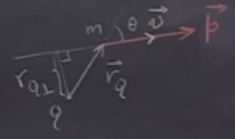
\includegraphics[scale=0.7]{\pIImages/lec20_angular_momentum}
\end{center}

The definition is then that the angular momentum relative to the point Q is

\begin{equation}
\vec{L_Q} = \vec{r_Q} \times \vec{p} = (\vec{r_Q} \times \vec{v}) m
\end{equation}

The direction can be found via the right-hand rule (into the blackboard in this case), and the magnitude is

\begin{equation}
|L_Q| = m v r_Q \sin \theta
\end{equation}

where, in shorthand notation, $r_Q \sin \theta = r_{\perp Q}$ may also be used. $\theta$ is, as usual in these cases, the smallest angle between the two vectors. This magnitude follows directly from the definition of the cross product, $\vec{a} \times \vec{b} = a b \sin \theta$. Also, $m(\vec{a} \times \vec{b}) = m a b \sin \theta$; nothing strange there.

Things do start to get strange now, however. We can consider the angular momentum as seen from a different point, call it C, that is located anywhere along the line of the velocity vector (i.e. a point where the object has been, or will be, assuming the direction of the velocity does not change).\\
Here, because $\vec{r_{C}} \times \vec{v} = \vec{0}$, since the two are parallel and cross products have a $\sin \theta$ term in them, the angular momentum relative to C is zero.\\
If we instead choose a point D above this line, the angular momentum relative to this new point D even has the opposite direction as the angular momentum relative to point Q.

This is then clearly a major difference between angular momentum and ``regular'' momentum (linear momentum, or translational momentum; both names are used).\\
Linear momentum has a certain value that is fixed for a certain reference frame. (We can still find reference frames where it is zero, or even opposite in direction, but that is a different discussion.)\\
Angular momentum, however, depends not only on your reference frame, but also on your point of origin. If you consider the origin to be at yourself, and look at a moving object, its angular momentum depends on where you stand, not only on your reference frame.

Consider the case of an object moving along a parabola (or a similar shape -- with or without air drag). It starts out at a point C, and first moves up, and then falls back down, all the while it moves at constant velocity along the x axis.

At time $t = 0$, the object is located at point C, so the angular momentum at time $t = 0$ is clearly 0: $\vec{r_C} = 0$ makes the cross product zero.\\
At any later time, however, there is a nonzero position vector, and a velocity vector that is not parallel to the position vector. Therefore, angular momentum is constantly changing. This does make sense, since the velocity vector is constantly changing.

There are, however, cases where a constantly changing velocity does not imply that angular momentum is changing.

Consider the Earth, going around the Sun, in a circular orbit. (The true orbit is elliptical, but we have not introduced such orbits yet.)

We define the point C to be at the center of the orbit, i.e. at the center of the Sun. We then have the position vector $\vec{r_C}$ to the Earth, which itself has a velocity vector $\vec{v}$, which is always changing, to be tangential to the orbit. The orbital speed $v$ is constant, however.

\begin{center}
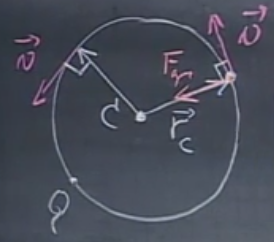
\includegraphics[scale=0.7]{\pIImages/lec20_orbit_torque}
\end{center}

The direction of the angular momentum relative to point C, $L_C$, is easy to find via the right hand rule; it is out of the page. The magnitude is found as

\begin{equation}
|L_C| = m v r_C \sin \theta
\end{equation}

However, the angle $\theta$ between the position vector and the Earth's velocity vector is always 90 degrees. Therefore, the sine of that angle is always 1, and $|L_C| = m v r_C$.\\
A while later in time, the exact same thing still applies. The velocity vector has changed direction, but the direction of the cross product remains constant. $\theta$ remains 90 degrees, and so the magnitude remains.\\
The angular momentum, relative to point C, is constant.

What about relative to some other point $Q$, which is on the Earth's orbital circle? It is clearly changing with time. When the Earth is \emph{at} that point, it must be zero, since $r_Q = 0$. When the Earth is \emph{not} at that point, it must be nonzero, as $\vec{r_Q} \times \vec{v} \neq 0$.

In other words, angular momentum is \emph{conserved} relative to point C, but is \emph{not} conserved relative to any other point!

\subsection{Torque}

Let's now have a look at torque. If angular momentum is the rotational analogue of linear momentum, torque is the rotational analogue of force.

We can write down an expression for the angular momentum relative to some point Q (which can be any point whatsoever), and then take the time derivative of that expression. We will need to use the product rule, though that is not a particularly difficult task:

\begin{align}
\vec{L_Q} &= \vec{r_Q} \times \vec{p}\\
\frac{dL_Q}{dt} &= \frac{d\vec{r_Q}}{dt} \times \vec{p} + \vec{r_Q} \times \frac{d\vec{p}}{dt}
\end{align}

The first of the two terms is the cross product between $\vec{v_Q}$ and the momentum vector of the Earth, but because that velocity and the momentum vector are always parallel ($\vec{p} = m \vec{v}$), that term is zero. What remains is a term that is the position vector cross the net force on the Earth, since $\displaystyle \vec{F} = \frac{d\vec{p}}{dt}$.

The quantity $\displaystyle \frac{d\vec{L_Q}}{dt}$ is known as the \emph{torque} relative to point Q. We use the symbol $\tau$ (Greek letter tau) for torque:

\begin{equation}
\vec{\tau_Q} = \frac{d\vec{L_Q}}{dt} = \vec{r_Q} \times \vec{F}
\end{equation}

Torque is also known as moment or moment of force, and may also be translated to something along the lines of ``turning moment'' in some other languages. $M$ or $N$ are other symbols used for torque, especially when it is called moment.\\
Note that torque, exactly as with angular momentum, is also relative to a point! We cannot, in general, talk about ``the'' torque on an object, without specifying our point of origin. Therefore, I used $\vec{\tau_Q}$ above, to show that we are talking about the torque relative to that same point Q.

The torque is the amount of ``twisting'' a force provides. Consider a nut and a wrench. The further out you grip the wrench, the easier it is to loosen a nut/bolt. That is because you are increasing the position vector $\vec{r_C}$, and the torque is proportional to this length. Needless to say, if you increase the amount of force you exert, the torque also increases.

The torque is also proportional to $\sin \theta$ (because of that term in the cross product $\vec{r} \times {F}$) which is quite intuitive. Only the force that is perpendicular to the wrench causes any turning of the nut. If the force is entirely parallel, you are just pushing or pulling on it the nut/bolt, and it will certainly not turn because of that force. For angles in between the extremes of 0 and 90 degrees, the closer you are to a perpendicular angle, the stronger the torque is.

If there is a net torque on an object (relative to a point), angular momentum (relative to that same point) must change. With zero net torque, angular momentum is conserved.\\
There is a clear parallel to conservation of linear momentum here: if there is a net force on an object, its momentum must change. With no net force, momentum is conserved.

Now, consider the case of the Earth orbiting the Sun again. The force vector is always inwards, and it is therefore always anti-parallel to $\vec{r_C}$. The cross product $\vec{\tau_C} = \vec{r_C} \times \vec{F}$ is always zero! This is the same result as we found earlier, but now we know why that must be.

Of course, if we calculate the torque at point $Q$, or any other point for that matter, the torque will not be zero, and will also not be constant. We will come back to what is so special about this center point $C$.

\subsection{Spin angular momentum}

So far, we have only really talked about the angular momentum of a point mass, moving through space (even if one such ``point mass'' was the Earth!). We will now consider objects of nonzero size, that rotate around their center of mass. For example, a rotating disk. It has a radius $R$, a mass $M$, and rotates about point C which is its center of mass.

\begin{center}
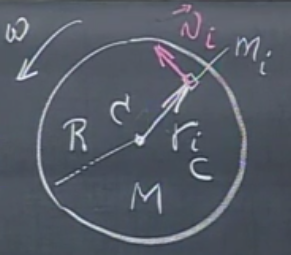
\includegraphics[scale=0.7]{\pIImages/lec20_spin_angular_momentum}
\end{center}

We can now, as we did for the moment of inertia among other things, split the disk up into small mass elements $m_i$. Each such element moves with velocity $v_i$. However, as before, we want to express this velocity in terms of $\omega$, since the velocity is a function of the distance to the center, whereas $\omega$ is not. We can use $v_i = \omega r_{iC}$; clearly we need to have that radius in there, anyhow.

The magnitude of the angular momentum for this tiny mass element alone is $L_{Ci} = (\vec{r_iC} \times \vec{v_i}) m_i = m_i r_{iC} v_i = m_i r_{iC}^2 \omega$. There is no $\sin \theta$ term since $\theta$ is always 90 degrees, and so $\sin \theta = 1$.\\
The direction can be found by the right-hand rule as usual, and is out of the blackboard (or page) in this case.

Now, in order to find the total angular momentum, we must sum up the angular momenta of all these tiny mass elements:

\begin{equation}
L_{disk_C} = \sum_i m_i r_{iC}^2 \omega = \omega \sum_i m_i r_{iC}^2 = I_C \omega
\end{equation}

If we factor out $\omega$ of the sum, since it is common to all elements, all that remains in the sum is $\sum_i m_i r_{iC}^2$, which as we have seen previously is just the moment of inertia for the disk. Therefore, we can find the angular momentum of the disk relative to point C as $I_C \omega$.

What is now remarkable is that this value is the angular momentum relative to \emph{all} points anywhere in space, not just relative to point C. This is true because of, and only in the cases where, this is a rotation around the center of mass.

$I_C \omega$ is referred to as the spin angular momentum, and is an intrinsic property of an object, regardless the origin you choose.\\
It is valid for objects of all shape, not only disks, as long as the rotation is about the center of mass.
(Everything I find about the term ``spin angular momentum'' is about quantum mechanics, however. I'm unsure whether this is a common terminology or not, but it appears not.)

$I_C \omega$ for the disk then gives us $\displaystyle L_{disk_C} = \frac{\omega}{2} M R^2$.

This concept is of course very handy. In the case of an object spinning around its center of mass, we can now talk about \emph{the} angular momentum of that disk, without having to specify any point of origin.

\subsection{Derivation/proof of spin angular momentum}

Let's prove that we can indeed don't need to measure spin angular momentum relative to some point, by calculating the angular momentum of an object spinning about its center of mass (where the center of mass is stationary, relative to the point). I call this point Q. In the end, everything relating to this point will have turned out to be zero.

First, let's make some definitions; this isn't as bad as it looks.

$\vec{R_{cm}}$ is the position vector from point Q to the center of mass (the center of the rotation)\\
$\vec{R_i}$ is the position vector from point Q to each mass element $m_i$\\
$\vec{V_i}$ is the velocity vector of each mass element $m_i$ seen from point Q\\
$\vec{r_i}$ is the position vector from the center of mass to each mass element $m_i$\\
$\vec{v_i}$ is the velocity vector from the center of mass to each mass element $m_i$

So capital letters are vectors from point Q, and lowercase are from the center of mass/relative to the mass elements themselves. Keep that in mind and this shouldn't be that hard to read.

%TODO: add image
%\begin{center}
%\includegraphics[scale=1.2]{\pIImages/spin_angular_momentum_proof}
%\end{center}

Via vector addition, we have

\begin{equation}
\vec{R_i} = \vec{R_{cm}} + \vec{r_i}
\end{equation}

By taking the time derivative of the above equation, we find $\vec{V_i} = \vec{V_{cm}} + \vec{v_i}$.\\
The definition of angular momentum relative to point Q is the sum of the angular momenta of each tiny mass element as seen from point Q, which is found as $\vec{R_i} \times \vec{P_i}$.

\begin{equation}
L_Q = \sum_i \vec{R_i} \times \vec{V_i} m_i = \sum_i (\vec{R_{cm}} + \vec{r_i}) \times (\vec{V_{cm}} + \vec{v_i}) m_i
\end{equation}

The entire point of this proof is that we have pure rotation about the center of mass, so $V_{cm} = 0$. Expanding the sum out and removing everything multiplied by $V_{cm}$, we find

\begin{equation}
L_Q = \sum_i \vec{R_{cm}} \times \vec{v_i} m_i + \sum_i \vec{r_i} \times \vec{v_i} m_i
\end{equation}

$\vec{R_{cm}}$ doesn't change during the summation, since it points to the center of mass, not to each mass element (not to mention $V_{cm} = 0$, so it's a constant):

\begin{equation}
L_Q = \vec{R_{cm}} \times \sum_i \vec{v_i} m_i + \sum_i \vec{r_i} \times \vec{v_i} m_i
\end{equation}

We can now see that the first term in zero: the sum of the momenta $\vec{v_i} m_i$ is zero in the center of mass frame (it is also called the center of momentum frame, or zero momentum frame). The term that remains can be shown to be equivalent to $I_{cm} \omega$, which is really derived in the section prior to this one (for a disk, at least).\\ 
For a rigid object seen from the center of mass, $\vec{r_i}$ and $\vec{v_i}$ are always perpendicular. We can get evaluate the cross product (since we only care about magnitude; the direction is certainly the same as the $\vec{\omega}$): $|\vec{r_i} \times \vec{v_i}| = r_i v_i \sin (\pi/2) = r_i v_i$.\\
Next, we apply $v_i = \omega r_i$:

\begin{equation}
L_Q = \sum_i r_i v_i m_i = \sum_i r_i (r_i \omega) m_i = \omega \sum_i r_i^2 m_i
\end{equation}

The sum is now simply the moment of inertia about the center of mass:

\begin{equation}
L_Q = L_{cm} = \omega \sum_i r_i^2 m_i = I_{cm} \omega
\end{equation}

And we are done! Everything specific to point Q has disappeared, and we end up with this simple result. Since there was nothing specific whatsoever about the point chosen, this holds for all points.

\subsection{Back to spin angular momentum}

The Earth has both a spin angular momentum and an orbital angular momentum due to its motion around the Sun. The spin angular momentum is quite easy to find as $I_C \omega$.\\
The moment of inertia for a sphere spinning about its center of mass is $\displaystyle \frac{2}{5} M R^2$, derived in the previous lecture. Using $R_{Earth} = 6400$ km and $T = 86400$, which translates into $\omega \approx \SI{7.2722e-5}{rad/s}$, 

The spin angular momentum of the Earth is then

\begin{equation}
\left(\frac{2}{5} (\SI{5.972e24}{kg}) (\SI{6400e3}{m})^2\right) (\SI{7.2722e-5}{rad/s}) = \SI{7.11e33}{kg m^2 s^{-1}}
\end{equation}

I'm not sure what units to use; the dimension is $\text{kg m}^2 \text{ s}^{-1}$, which is equivalent to $\text{N}\cdot\text{m} \cdot \text{s}$ and $\text{J} \cdot \text{s}$. Presumably one set of units is more common than the others!\\
... Coming back to this section after having finished this week's lectures, I would guess that the newton-meter-second is the most common unit (in general) for angular momentum. If a torque of 1 Nm acts for 1 second, the angular impulse (the change in angular momentum) is (1 Nm)(1 s) = 1 Nms. In this particular case (above), though, we have the units explicitly in terms of kg, $\text{m}^2$ and rad/s.

Anyhow.
The orbital angular momentum around the Sun, relative to the center of the orbit, is

\begin{equation}
L_C = (|\vec{r_C} \times \vec{v}|) m = m r_s \frac{2 \pi r_s}{T_{orbit}} = \frac{2 \pi m r_s^2}{T_{orbit}}
\end{equation}

where $r_s$ is the radius of the Earth's orbit, about 150 million km, or \SI{1.5e11}{m}. The mass $m$ is $\SI{5.97e24}{kg}$. $T_{orbit} \approx 86400 \times 365$, so
This then gives us \SI{2.677e40}{kg m^2 s^{-1}}.

The ratio of the two, with spin angular momentum on top, is about $\num{2.66e-7}$.

\subsection{Conservation of angular momentum: an experiment}

Consider a person, standing on a plate that is free to rotate, like this:

\begin{center}
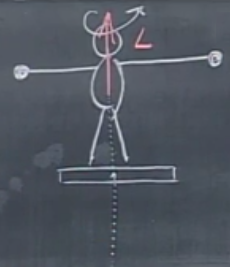
\includegraphics[scale=0.7]{\pIImages/lec20_cons_angular_momentum}
\end{center}

In his hands, he holds two weight of mass $m \approx 1.8$ kg (each). The mass of the person, including the weights plus the turntable itself, is $M \approx 75$ kg.
In this counterclockwise rotation, seen from above (clockwise from below, though I find it easier to see this from above), the angular momentum vector will be upwards.

In a case like this, we have a rotation about a center of mass. Angular momentum has a value found simply by $I_C \omega$, and it will be conserved, after the initial push to get the person rotating. When rotating, these weights can be moved either close to his body, or as far out as his arms can reach. Clearly, this does not cause an \emph{external} torque, so angular momentum $L_C$ must be conserved.

However, $I_C$, the moment of inertia, will change! Since $L = I_C \omega$, and $I_C$ will go down, $\omega$ must go up -- there is no other way for the conservation to hold.

In a semi-quantitative calculation, we can approximate the professor as a cylinder, with radius $R = 0.2$ m. The cylinder has a mass of 75 kg\footnote{I think it should be 75 kg minus the 2 times 1.8 kg, but these numbers will clearly not be very accurate either way.}, and so has a moment of inertia of about $\frac{1}{2} M R^2 = \SI{1.5}{kg m^2}$.

Now, if we ignore the weight of the professor's arms, when stretching them out, two additional point masses are added, at arm's length from the axis of rotation. The moment of inertia for each weight is about $m r^2 = \SI{1.5}{kg m^2}$, assuming an arm length of 90 cm.\\
When his arms are stretched out, we then find the total moment of inertia to be the roughly 1.5 from the professor's body, plus another 3 from the weights! This difference of a factor of 3 (4.5/1.5) when pulling the weight in close causes a difference in $\omega$ of a factor of three, so the change in the angular velocity is very apparent!

\subsection{Conservation of angular momentum (in general, and in stars)}

Let's look at conservation of angular momentum in a similar way to how we treated linear momentum.

Say we have a group of objects interacting: stars, interacting gravitationally, point particles of any kind, objects connected together with springs, etc. There can be any kind of internal interactions between these, including collisions, internal friction, explosions/supernovae, and so on.\\
Because all internal forces will cancel out, there can never be any net internal torque relative to any point Q we choose. In the absence of a net \emph{external} torque, angular momentum will be conserved. In the presence of a net external torque, angular momentum will change according to

\begin{equation}
\frac{d\vec{L_Q}}{dt} = \vec{r_Q} \times \vec{F_{Ext}} = \vec{\tau_{Q,Ext}}
\end{equation}

... for the entire system as a whole. The angular moment of any one object \emph{inside} that system is, just as with linear momentum, \emph{not} conserved. Essentially, they can ``trade'' angular momentum with each other, but the net angular momentum of the entire system cannot change.

Similar to the experiment the professor did, reminiscent of ice skaters, stars can also shrink, and have their moments of inertia go down (since $I \propto R^2$), which means that the star's angular velocity must increase: $L = I \omega$ must be constant in the absence of a net external torque.

In a star, 	the nuclear fusion going on causes forces that want to expand the star outwards. However, there is also gravity, which does what it can to collapse the star towards its center. In all stars that are actively ``burning'' fuel, these two forces are balanced out.

What now happens when the fuel runs out, and fusion can't continue on? This won't happen for about 5 billion years for our Sun, but it happens all the time for other stars, considering the amount of stars in the observable universe. There are three possible end products of stars.

The first is that the star becomes a \emph{white dwarf}. They have radii of about $10^4$ km, not too far from the radius of the Earth, and a mass of about half our Sun's mass. Our Sun will end up as a white dwarf far in the future.\\
We can see that the density of such an object must be very high, with half the Sun's mass, but a volume almost comparable with that of the Earth. The density becomes on the order of $\SI{1e6}{g/cm^3}$.

The second possibility is that the star becomes a \emph{neutron star}, a very interesting type of celestial object. They have radii on the order of 10 kilometers -- less than many cities -- yet a mass typically in the range 1.4 to 3.2 solar masses! This causes a ridiculous density of some $10^{14} \text{ g/cm}^3$. Neutron stars are so named because they are thought to consist largely of neutrons. In some ways, they are like enormous nuclei.\\
The Crab pulsar, which we discussed earlier, is a neutron star. In fact, all pulsars are neutron stars. Not all neutron stars are pulsars, however, since they do stop rotating sooner or later, at which point they no longer pulse. Also, pulsars are mostly defined by the fact that they pulse towards the Earth, so the vast majority of such neutron stars may go unnoticed, since their light beams are unlikely to be pointed towards us.

Finally, the third possibility is that the star becomes a \emph{black hole}, an even more bizarre type of celestial object. This can only happen for stars that are more massive than about three solar masses.\\
Black holes will not be covered in this lecture, but will be in the future.

When a star collapses, due to the lack of outwards pressure, a huge amount of gravitational potential energy is converted to kinetic energy, as the mass of the star falls inward. That energy is ultimately turned into heat and radiation.\\
In addition, because the moment of inertia is reduced as the mass moves inwards, the rotational period of the star increases, often dramatically. (Especially for neutron stars, see below.)

Our Sun will not become a neutron star, as it is not massive enough, but let's do some calculations on it anyway, just to get a feeling for some numbers. The radius of the Sun is about 700 000 km, while that of a neutron star might be about 10 km.\\
The mass is about $\SI{2e30}{kg}$. In moving all this mass inwards, there is a huge loss in gravitational potential energy, on the order of $\Delta U = 10^{46}$ joules.\\
This is converted to kinetic energy, and then conserved into heat and radiation, etc.

This energy is on the order of \emph{100 times more} than the Sun releases in its \emph{10 billion year} lifetime -- and this explosion releases that energy in a matter of seconds, rather than billions of years! This is what we call a supernova. (There are different types of supernovae; this is one of them.)

``A white dwarf, with a mass of $\SI{2.8e30}{kg}$ and a radius of about 10 000 km implodes (via gravitational collapse) to becomes a neutron star of the same mass with a radius of about 10 km. The rotational period of the white dwarf was $T_i = 10$ hours. What will the rotational period of the neutron star be? For simplicity, assume that the mass density in both the white dwarf and the neutron star is uniform.''

Okay, so let's first convert these numbers a little. The initial radius is $10000\times10^3 = 10^7$ m, and the final radius $10^4$ m. The initial period is $T_i = 36000$ seconds.

$\displaystyle L = I \omega = I \frac{2 \pi}{T}$ is conserved, so when $I$ goes down, $T$ must go down by the same factor. $I \propto R^2$, and the change in $R$ is a factor $10^3$, so the change in $R^2$ in a factor of $10^6$. The time period becomes $T = 36000 \times 10^{-6} = 0.036$ seconds (27.77 Hz, up from $\SI{2.77e-5}{Hz}$!).

\subsection{More on supernovae, pulsars and neutron stars}

The idea behind these notes is not to provide a transcript, and as such, as I do now and then, I recommend simply watching this part of the lecture at this point. There is quite a bit of information, but most of it works better in context in the video, so I see little point in copying it down here almost verbatim!

\section{Lecture 21: Torque}

The lecture begins with a review of the last week. I didn't find anything in particular to take notes of again. After all, being able to review is sort of the point of these notes!

Still, here are a few equations given:

\begin{align}
\vec{L_Q} &= \vec{r_Q} \times \vec{p}\\
\vec{\tau_Q} &= \vec{r_Q} \times \vec{F}\\
\frac{d\vec{L_Q}}{dt} &= \vec{\tau_{Q,Ext}}
\end{align}

The last equation is often used for a system of objects, thus the ``external'' qualifier. With no net \emph{external} torque, angular momentum in conserved... relative to that point Q, since that may be the only point with zero torque.

In rotation about some point Q, we can write a variant of Newton's second law, that relates torque with moment of inertia and angular acceleration (rather than relating force with mass and linear acceleration), as well as a relation that relates angular momentum with moment of inertia and angular velocity (rather than relating linear momentum with mass and linear velocity):

\begin{align}
|\tau_Q| &= I_Q\ \alpha_Q \text{, where $\alpha = \ddot{\theta}$, $\omega_Q = \dot{\theta}$}\\
|L_Q|    &= I_Q\ \omega_Q
\end{align}

In the special case of a rotation about the center of mass of an object, the angular momentum is instead an intrinsic property of that object, and it \emph{no longer matters} which point Q we choose. In that case

\begin{equation}
|L_{cm}| = I_{cm} \omega_{cm}
\end{equation}

In all other cases, it is crucial to specify the point of origin chosen, since angular momentum depends on not only your reference frame, but also the point of origin.

Let's now look at a case where angular momentum is conserved for exactly one point, but is not conserved for any other.\\
We have a rod, that we rotate about a point P, which is a distance $d$ from the center of mass C. It has a mass $M$ and a length $\ell$, and we rotate it with an angular velocity $\omega$.

\begin{center}
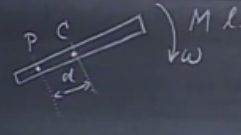
\includegraphics[scale=0.7]{\pIImages/lec21_rod}
\end{center}

The moment of inertia for rotation about the center of axis of a rod of uniform density is $\displaystyle \frac{1}{12} M \ell^2$, so angular momentum relative to point P is

\begin{equation}
|L_P| = I_P \omega = \left(\frac{1}{12} M \ell^2 + M d^2\right) \omega
\end{equation}

where the $M d^2$ term is added because of the parallel axis theorem.

There will be a force acting on the ruler at point P, as well as one acting on the pin (that it rotates around) \emph{by} the ruler. We can show this by analogy. Consider a massless rod, with two equal masses on each end. We rotate this rod about the center of mass, which is also the center of the rod. There is a centripetal force inwards on each of the masses, of equal magnitude since the masses are equal and the distance from the point of rotation are equal (and the velocities of the masses are then also equal).\\
However, if we rotate the rod about a point that is closer to one of the masses, then the centripetal force on that mass is smaller, but the centripetal force no the other is larger, since they move in circles of different radius. (As the point of rotations comes closer to one of the masses, it almost doesn't rotate at all, but rather spins about its axis.)

For this reason, there will be a force on the pin (and a reaction force from it) at point P in the ruler. The \emph{torque} relative to point P is zero, however: the force is along the ruler, and the position vector in $\vec{r} \times \vec{F}$ is also along the ruler.

Since $|\vec{\tau_P}| = 0$, angular momentum is conserved in this case. It would not be if we chose any other \emph{stationary} point, however.

Let's now rotate the same ruler about the center of mass C. The problem is now symmetric, like the case with the two masses mentioned above, and so there is now no net force on the pin/due to the pin. With no net force, $\vec{\tau_Q} = \vec{r_Q} \times \vec{F}$ must be zero for \emph{all} points Q, since $F = 0$. Therefore, in this case, angular momentum is conserved relative to \emph{all} points, as there is no net torque relative to \emph{any} point. The magnitude of the angular momentum for the rotation about the center of mass is then simply $I_C \omega$, which for a rod is

\begin{equation}
|L_{CM}| = \frac{1}{2} M \ell^2 \omega
\end{equation}

for all points in space.

\subsection{Off-center impulse: translation and rotation}

Let's now consider a ruler, lying flat on a frictionless table. It has a uniform mass density, and so its center of mass C is located at the geometric center. We give it an impulse $I$, in other words, a force that acts for a certain amount of time (a very short amount of time in this case, but that is not strictly necessary for this to hold).

\begin{center}
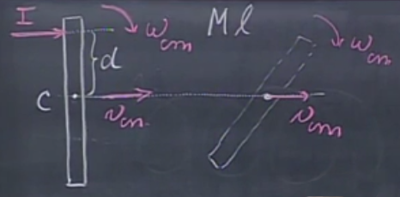
\includegraphics[scale=0.7]{\pIImages/lec21_ruler_rotation}
\end{center}

What will happen? Clearly, it is going to move towards the right. It will also rotate, assuming you don't aim for the center of mass (i.e. assuming $d \neq 0$).

The object \emph{must} rotate about its center of mass -- anything else is impossible. If it were to rotate about a point offset from the center of mass, then the center of mass would have to move in a spiral-ish motion. Due to conservation of (linear) momentum, the center of mass must have a constant velocity (meaning both magnitude and direction are constant!) after the initial push, which is only possible if any rotation is about the center of mass.\\
(Keep in mind that this is assuming a frictionless table. On a real table, where $\mu$ likely differs at different points, the results may also therefore differ: there is then an external force that may vary in unpredictable ways!)

That much is fairly intuitive, in my opinion, but what's interesting that the distance $d$ from the center of mass where the impulse happens does not affect the velocity of the center of mass. For a given amount of momentum given by the impulse, the velocity of the center of mass is constant, regardless of $d$. I find this nonintuitive, but it is still easy to see mathematically.

$\vec{p} = m \vec{v_{cm}}$ must hold, and since initial momentum is 0, $\vec{p} = \vec{I}$ after the initial push. Nowhere in the equation does $d$ appear -- the equation in question is valid for any isolated system, regardless of shape and place where the force is applied, as long as it is rigid.\\
Since $\vec{p} = \vec{I}$, the above equation also says that

\begin{equation}
\vec{v_{cm}} = \frac{\vec{I}}{m}
\end{equation}

$\omega$, on the other hand, clearly depends on the distance $d$. If $d = 0$, then $\omega = 0$; that much is clear. It is also clear that $\omega$ grows as $d$ grows. The reason is that the amount of torque (relative to the center of mass) provided depends on $d$ and the amount of force provided during the impulse. (The amount of angular impulse, i.e. change in angular momentum, depends on the average torque and the time, $J = \tau \Delta t$, just like how the linear impulse is given by $I = F \Delta t$.)\\
($\omega$ was calculated in this week's homework: week 9/homework 7, problem 9.)

However, note that if we instead look at the torque relative to a point P on the line of the impulse, i.e. a distance $d$ up from the center of mass, this torque is zero! Zero torque means angular momentum will be conserved, and so angular momentum \emph{relative to point P} is zero not only before, but also after the object starts to rotate. It is therefore conserved, unlike angular momentum relative to the center of mass!

\subsection{Physical pendulum}

Let's have a look at a different ruler. We previously derived an equation describing the motion of a simple pendulum, as a simple harmonic oscillator. We made some unrealistic approximations, however, including a massless string and a point mass hanging from it.\\
We will now consider a related yet different type of oscillator, called a physical pendulum.

In this case, we have a ruler, though the solution is valid for other shapes as well. We drill a hole through it at point P, and hang it on a small pin. The point P is located a distance $b$ from the center of mass, point C.

\begin{center}
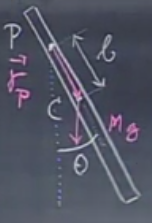
\includegraphics[scale=0.7]{\pIImages/lec21_physical_pendulum}
\end{center}

The ruler makes an angle $\theta$ with the vertical. Using the concept of the center of mass, we can consider gravity acting only at the center of mass; the magnitude is $M g$, where $M$ is the total mass of the ruler.

If we choose to use point P as our origin, our lives become much easier. There will be a force at point P, but if we choose it as our origin, we do not have to worry about those forces, since the torque due to those forces will be zero: $\vec{\tau_P} = \vec{0} \times \vec{F}$, since the first term is the position vector from P to P.

There is a torque that matters, relative to point P, however: the torque due to gravity acting on the center of mass. The distance $b$ acts as a lever arm, and the torque is given as the cross product between the distance and the force. The torque can also be found as $I_P \alpha$, as we saw earlier.

\begin{equation}
|\vec{\tau_P}| = \vec{b} \times \vec{F_g} = M g b \sin \theta = - I_P \alpha
\end{equation}

The torque is always trying to restore things back to equilibrium, which gives us a minus sign, just as how we used $- k x$ for the force when deriving the equation governing a spring oscillator. Note that we have used the Newton's second law equivalent for torques: $F = m a \Rightarrow \tau = I \alpha$.

$\alpha = \ddot{\theta}$ by definition, in a different form of notation. Now, using the small angle approximation that we have used several times earlier, $\sin \theta \approx \theta$. This is fairly valid for small angles; at 5 degrees, the difference is less than 0.15\%; at 10 degrees, the difference is about 0.5\%.\\
By using this approximation, and making the substitution for $\alpha$, we have

\begin{align}
M g b \theta &= - I_P \ddot{\theta}\\
I_P \ddot{\theta} + M g b \theta &= 0\\
\ddot{\theta} + \frac{M g b}{I_P} \theta &= 0
\end{align}

A-ha! This has the exact form of a simple harmonic oscillator! We already know the solutions; the square root of the stuff multiplying $\theta$ gives us the angular frequency $\omega$, etc:

\begin{align}
\theta(t) &= \theta_{max} \cos(\omega t + \phi)\\
\omega    &= \sqrt{\frac{M g b}{I_P}}\\
T         &= \frac{2 \pi}{\omega} = 2 \pi \sqrt{\frac{I_P}{M g b}}
\end{align}

Keep in mind that because $I_P \propto M$, this is in fact independent on the mass, just as with a simple pendulum. We can substitute in the value for $I_P$, in which case we transform the general result, above, into a result that only holds for a rod.\\
$I_P = \frac{1}{12} M \ell^2 + M b^2$ via the parallel axis theorem. Making that substitution,

\begin{align}
\omega    &= \sqrt{\frac{g b}{\frac{1}{12} \ell^2 + b^2}}\\
T         &= \frac{2 \pi}{\omega} = 2 \pi \sqrt{\frac{\frac{1}{12} \ell^2 + b^2}{g b}}
\end{align}

Again, note that these results are now only valid for the case of a rod.

As a side note, we can also write for the angular acceleration $\alpha = \dot{\omega}$. This is a very confusing thing to do, however! The omega in the previous sentence is the \emph{angular velocity}, i.e. how fast the angle is changing with time, analogous to the velocity $v$ for linear motion. This omega is \emph{constantly changing in time}, and has a minimum at $\theta_{max}$, as the pendulum reverses direction, and a maximum at $\theta = 0$.

On the other hand, the $\omega$ used in the cosine above, and the only one I have mentioned prior to the paragraph above to avoid confusion, is the \emph{angular frequency}, $\displaystyle \omega = \frac{2 \pi}{T}$. That $\omega$ is a \emph{constant}, and is only related to how many oscillations the pendulum completes per second. This sentence marks the last mention of the angular velocity $\omega$ in this section; only the one that represents angular \emph{frequency} will be used from here on.

Let's try to calculate the approximate period, including the uncertainty, of this pendulum when $\ell = 1.00$ m and $b = \SI{0.400(2)}{m}$, i.e. the uncertainty is 2 mm or 0.2 cm.

In the ideal case, the number we find by plugging in the numbers is $T = \SI{1.5497}{s}$, using $g = \SI{10}{m/s^2}$.\\
The largest possible time should be when $\ell$ and $b$ are both maximized, which gives $T = 1.556$ s. On the other side of things, the smallest possible period is about $T = 1.543$ s.

The uncertainty is about 0.0065 seconds or so; call it 0.01 s.\\
It turns out the professor used $g = \SI{9.8}{m/s^2}$, which is probably a good idea if you're going to time this in the real world. In either case, he found $T = 1.565$ seconds, which is very close to these numbers.

This is then demonstrated, and the timing indeed works out.

Next, we look at the same type of oscillation, but we use a hula hoop as the pendulum, instead of the ruler. The derivation is almost identical, and except for some variable names, we can still use the general equation we found earlier.

The center of mass of the hoop is at the geometric center, i.e. in the middle of empty space. We again hang it on a pin, at point P, which clearly is at the very top of the hoop.

\begin{center}
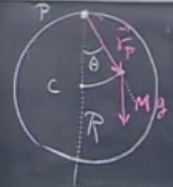
\includegraphics[scale=0.7]{\pIImages/lec21_hoop_pendulum}
\end{center}

As before, we consider the force of gravity as acting solely on the center of mass, with a force $M g$ downwards. Again as before, the position vector $\vec{r_P}$ acts as the lever arm, and the torque relative to point P is

\begin{equation}
\vec{r_P} \times \vec{F_g} = M g R \sin \theta = -I_P \ddot{\theta}
\end{equation}

As before, the torque must be equal to the negative of $I_P \alpha = I_P \ddot{\theta}$, using Newton's second law for circular motion. If we use the small angle approximation $\sin \theta \approx \theta$ again, and solve for $\ddot{\theta}$:

\begin{equation}
\ddot{\theta} + \frac{M g R}{I_P} \theta = 0
\end{equation}

Clearly, this is yet another simple harmonic oscillator! The only difference from the one we found for the rod is that we now used $R$ instead of $b$ for the distance to the center of mass; they are identical other than that non-detail.\\
The moment of inertia about point $I_P$ is the moment inertia about the center of mass $I_C$, plus $M R^2$ via the parallel axis theorem. $I_C$ is also $M R^2$ for a circular object with uniform mass distribution (all mass points are a distance $R$ away (derivation not shown), so $I_P = 2 M R^2$. That gives, using the solutions we found previously and using this new $I_P$,

\begin{align}
\theta(t) &= \theta_{max} \cos(\omega t + \phi)\\
\omega    &= \sqrt{\frac{g}{2 R}}\\
T         &= \frac{2 \pi}{\omega} = 2 \pi \sqrt{\frac{2 R}{g}}
\end{align}

This is the same result as we have found previously for a pendulum with a massless string, if we just call its length $2 R$! Quite neat, that they would have the same period.	

Time for an interesting lecture question.

\begin{center}
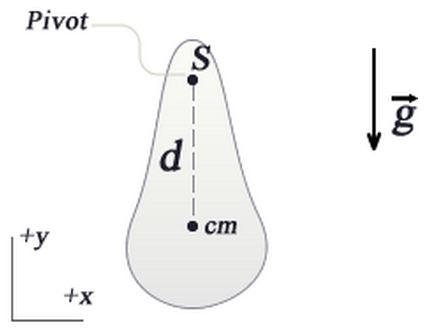
\includegraphics[scale=0.5]{\pIImages/lec21_physical_pendulum_2}
\end{center}

``A physical pendulum consists of a body of mass m contained in the xy-plane. The moment of inertia of the object about an axis perpendicular to the plane and passing through the object's center of mass is Icm.

The object oscillates in the xy-plane about the point S a distance $d$ from the center of mass as shown. What is the period of the pendulum for small angle oscillations where $\sin\theta \approx \theta$?''

Since they want the answer in terms of $I_{cm}$ (so that we don't need to actually calculate the moment of inertia) this should be fairly easy. In fact, we just use the general solution with $d$ as the distance between the point and the center of mass,

\begin{equation}
T = 2 \pi \sqrt{\frac{I_{S}}{m g d}}
\end{equation}

$I_S$ can be written as $I_{cm} + m d^2$, so

\begin{equation}
T = 2 \pi \sqrt{\frac{I_{cm} + m d^2}{m g d}} = 2 \pi \sqrt{\frac{I_{cm}}{m g d} + \frac{d}{g}}
\end{equation}

There is then a demonstration of the hula hoop, and a simple pendulum (an apple hanging on a lightweight string), to show that their periods are almost synchronized. (Most of the error likely comes from a small difference in length.)
